Le code que l'on veut exécuter sur la carte de développement doit être compilé pour celle-ci, puis placé sur un support de stockage. Ce code peut être un simple programme ou bien un système d'exploitation. Un système d'exploitation est un ensemble de programmes qui permettent de gérer les ressources d'un ordinateur. Il permet de gérer les périphériques, les processus, la mémoire, les fichiers, etc. Il permet aussi de fournir une interface entre l'utilisateur et la machine afin de faciliter l'utilisation de celle-ci. Un système d'exploitation permet aussi de standardiser ces interfaces afin de faciliter le développement de programmes et d'améliorer la portabilité de ceux-ci. Linux, Windows et MacOS sont des exemples de systèmes d'exploitation.

J'ai premièrement installé des images pré-compilées de Linux fournies par le fabricant de la carte, puis j'ai compilé moi-même le noyau Linux depuis son code source en réalisant une compilation croisée. Je me suis rapidement tourné vers l'étude des différentes versions de Linux compatibles avec la carte, car c'était l'un des deux seuls systèmes d'exploitation supportés par la carte, le second étant android. Android étant basé sur Linux, je ne voyais pas l'utilité d'en étudier les versions temps réels. 

\subsubsection{Installation d'une image pré-compilée}

Dans un premier temps, pour tester l'installation de Linux sur la carte de développement, j'ai utilisé une image de la distribution Ubuntu fournie par le fabricant \textit{96Boards} disponible sur leur site. 

Une distribution Linux est un ensemble de programmes qui forment un système d'exploitation. Il existe plusieurs distributions Linux, comme Ubuntu, Debian, Arch Linux, etc. Ces distributions sont souvent basées sur un même noyau Linux, mais possèdent des programmes différents. Par exemple, Ubuntu est basé sur Debian, et possède un ensemble de programmes différents de Debian.

Cette image se présente sous la forme d'une archive au format \texttt{.tar.gz}. Elle contient à la fois le \gls{bootloader}, le noyau Linux, et le système de fichiers. Cette image (\texttt{system.img}) peut alors être gravée (ou \textit{flashée}) sur une carte micro SD. 

Depuis un terminal, en se déplaçant dans le dossier de l'archive extraite, on exécute la commande suivante : 
\begin{lstlisting}[style=command, caption=Téléversement de l'image sur la carte microSD]
$ sudo dd if=system.img of=/dev/XXX bs=4M oflag=sync status=noxfer
\end{lstlisting}

Cette commande permet de copier le contenu de l'image sur la carte micro SD. Le paramètre \texttt{if} permet de spécifier le fichier source, ici l'image de la carte. Le paramètre \texttt{of} permet de spécifier le fichier de destination, ici la carte micro SD. Le paramètre \texttt{bs} permet de spécifier la taille des blocs de lecture et d'écriture. Le paramètre \texttt{oflag} permet de spécifier des options de copie, ici \texttt{sync} permet de synchroniser les entrées et sorties. Le paramètre \texttt{status} permet de spécifier le niveau de détail des informations affichées, ici \texttt{noxfer} permet de ne pas afficher le nombre de blocs transférés.

\subsubsection{Compilation de Linux depuis le code source}\label{sec:compilation-linux-source}

Afin d'utiliser une version de Linux différente de la version précompilé par le fabricant de la carte de développement, il faut premièrement se procurer le code source du noyau Linux. Celui-ci est disponible sur un dépôt de code \gls{git} hébergé par \textit{GitHub}. 

\gls{git} est un logiciel de gestion de versions décentralisé. Il permet de gérer l'historique des modifications d'un projet et de travailler à plusieurs sur un même projet. Chaque modification est enregistrée sous forme de \textit{commit}, c'est-à-dire un enregistrement de l'état du projet à un instant donné. Ces \textit{commits} sont ensuite regroupés en branches, qui sont des chemins de développement indépendants. Ces branches peuvent être fusionnées (ou \textit{merged}) entre elles afin de combiner les modifications de deux branches. Github est un site web qui permet d'héberger des dépôts de code \gls{git} et de faciliter le travail collaboratif. Un tel serveur peut aussi être hébergé localement, comme au LIAS avec \textit{GitLab}.

Le dépot de code, ou \textit{repository}, du noyau Linux est disponible à l'adresse \\ \texttt{https://github.com/torvalds/linux}, sous le profil du créateur de Linux : Linus Torvalds. Durant mon stage, j'étais libre d'utiliser le logiciel de gestion de version de mon choix, j'ai donc principalement utilisé \textit{git} en ligne de commande et j'ai parfois utilisé un client \textit{git} nommé \textit{GitKraken} afin d'explorer plus facilement les anciens \textit{commits} de certains projets comme \litmus.

Une fois le code source du noyau téléchargé, aussi appelé cloné, et en se déplaçant dans le dossier \texttt{linux} depuis un terminal, on peut alors procéder à la compilation. Pour mes premiers essais, j'ai décidé de compiler Linux pour une machine virtuelle que je fais tourner sur ma machine de travail.

Le noyau Linux est un programme ayant une compilation basée sur la configuration : cela signifie que certaines parties du code peuvent être rajoutées ou omises par le simple biais d'un fichier de configuration. Cette configuration se présente sous la forme d'un fichier \texttt{.config} qui doit être créé à la racine du noyau. Pour créer ce fichier, des utilitaires sont mis à notre disposition dans le noyau :
\begin{itemize}
    \item \texttt{make defconfig} : cet outil est utilisé pour générer une configuration par défaut. Ici l'architecture de la machine qui réalise la compilation est sélectionnée. Dans mon cas, éxécuter cette commande crée un fichier de configuration basé sur la config \texttt{'x86\_64\_defconfig'}.
    \item \texttt{make menuconfig} : cet outil permet d'éditer la configuration actuelle du fichier \texttt{.config} via une interface graphique. Ce menu permet aussi de rechercher des paramètres, de voir leur description et d'enregistrer différentes configurations.
\end{itemize}

\begin{figure}[H]
    \centering
    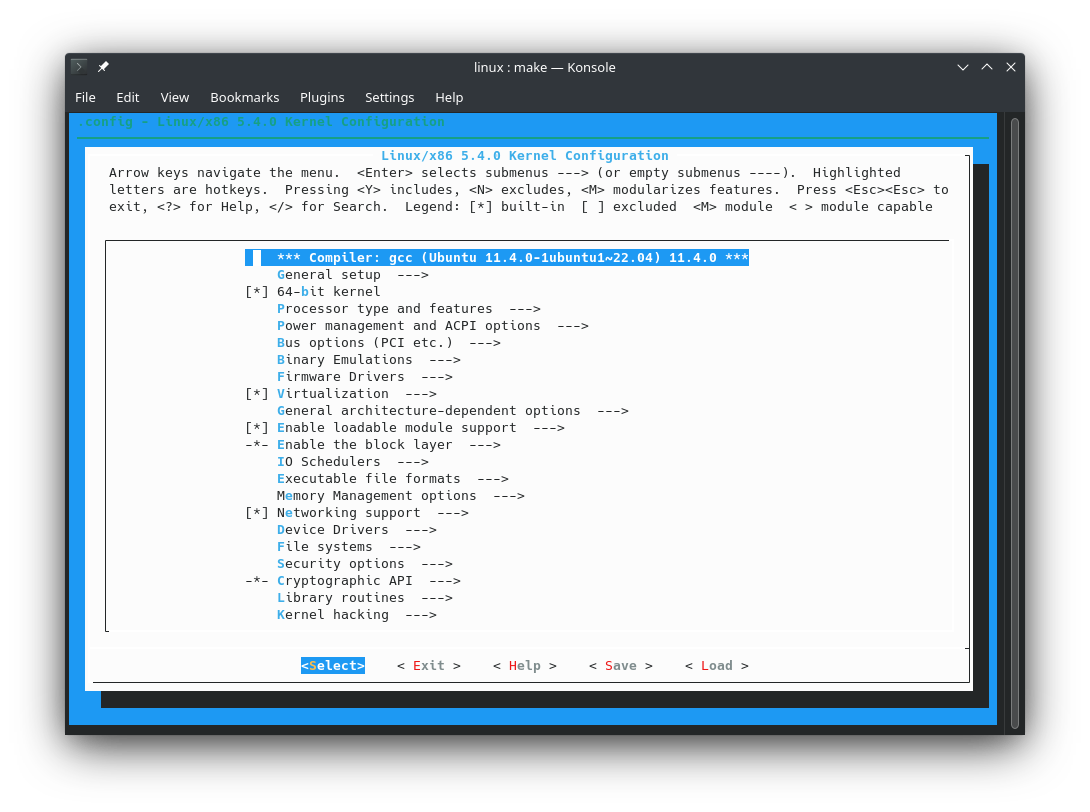
\includegraphics[width=0.65\paperwidth]{Images/make menuconfig.png}
    \caption{Interface de configuration du noyau}
\end{figure}

Le menu de \texttt{make menuconfig} s'appui sur les fichiers \texttt{Kconfig} présents dans les dossiers du noyau. Ces fichiers contiennent les différentes options de configuration du noyau. Par exemple, le fichier \texttt{Kconfig} du dossier \texttt{arch/x86/Kconfig} contient les options de configuration spécifiques à l'architecture \texttt{x86}. Ces fichiers sont écrits dans un langage propre à Linux, et sont ensuite compilés en un fichier \texttt{Kconfig} binaire. Ce fichier binaire est ensuite utilisé par \texttt{make menuconfig} pour afficher les différentes options de configuration. 

Une fois la configuration créée, nous pouvons passer à la compilation du noyau. Linux utilise l'utilitaire de compilation \textit{GNU Make} : il permet l'automatisation de la compilation, la gestion des dépendances et gère la personnalisation de la compilation de chaque dossier. Ces règles sont alors dictées par des fichiers \texttt{MakeFile} présents dans chaque dossier contenant des fichiers à compiler du projet.

Il est à noter que chaque distribution Linux possède un ensemble différent de programmes préinstallés, il faudra alors peut-être installer des programmes nécessaires a la compilation. Par exemple, installer \texttt{libelf-dev}, "une bibliothèque partagée qui permet de lire et écrire des fichiers ELF à un niveau élevé"\footnote{d'après la description sur packages.debian.org/fr/sid/libelf-dev}. 


\newpage %might need to be removed, but it's here to avoid a bad page break
\begin{lstlisting}[style=command, caption=Compilation sur plusieurs processeurs] 
$ make -j16
\end{lstlisting}

Le paramètre \texttt{-j 16} signifie que l'on veux exécuter la compilation avec 16 tâches en parallèle. Il est recommandé d'utiliser comme nombre de tâches le double du nombre de processeurs dans l'ordinateur qui réalise la compilation.

Par la suite, il sera parfois nécessaires de changer la version de Linux que je compile afin de tester si celle-ci fonctionne. Sur le dépôt de code de Linux, les différentes versions sont stockées sous forme d'un certain commit qui a été tagué afin de le retrouver. On peut alors changer de version en revenant à ce commit grâce à la commande \texttt{checkout} de \gls{git} : 
\begin{lstlisting}[style=command, caption=Retour sur un commit tagé]
$ git checkout v5.4
\end{lstlisting}
On peut avoir la liste de ces commits tagués de la manière suivante : 
\begin{lstlisting}[style=command, caption=Comment lister les tags]
$ git tag -l
\end{lstlisting}
On aura alors l'ensemble des tags de tout le dépôt de code, et on peut filtrer ces résultats, avec \texttt{grep} par exemple, si l'on veut retrouver une version particulière.

Bien que j'étais déjà familier avec git, cela m'a pris un certain temps afin de comprendre comment ce changement de version s'effectuait. La nuance que l'on ne changeait pas de branche dans le dépôt, mais que l'on revenait simplement au commit correspondant à la version était la plus compliquée à comprendre. Tout au long de ce stage, j'ai pu utiliser \gls{git} afin d'explorer comment certains projets ont été construits en remontant l'historique de leurs commits, mais j'ai pu aussi utiliser \gls{git} pour gérer le stockage du code que j'ai développé, qu'ils soient des outils ou des modifications du noyau.  


\subsubsection{Compilation croisée}

Nous ne pouvons malheureusement pas compiler directement le noyau Linux pour la carte de développement du fait de la différence de jeu d'instruction. Il faut donc réaliser une \textit{cross compilation} ou compilation croisée : c'est le fait de compiler un programme sur une architecture qui n'est pas celle de l'architecture cible.

\begin{figure}[H]
    \centering
    \begin{tikzpicture}[node distance=2cm, auto]
        % Rectangle 1: Ordinateur x86
    \node[draw, dashed, rectangle, align=center, minimum width=4cm, minimum height=5.5cm] (ordinateur){};
    \node[draw, rectangle, align=center, above=-0.75cm of ordinateur]{Ordinateur  \textbf{x86}};
    \node[above=-1.8cm of ordinateur] (kernelcode) {code du noyau};

    \node[below=0.75cm of kernelcode](compiledkernel){noyau compilé};

    \node[below=0.75cm of compiledkernel, align=center](fs){système de fichiers \\ Ubuntu + bootloader};

    \draw[->] (kernelcode.south) -- (compiledkernel.north) node [pos=0.5, right] {gcc-arm64};

    
    \draw[->] (compiledkernel.south) -- (fs.north);

    % Rectangle 2: Carte de développement
    \node[draw, dashed, rectangle, align=center, minimum width=4.5cm, minimum height=4.5cm, right=3cm of ordinateur] (carte) {};
    \node[draw, rectangle, align=center, above=-1.2cm of carte]{Carte de développement \\ \textbf{arm64}};
    \node[above=-3cm of carte, align=center] (kernelcode) {Lancement de Linux \\ basé sur la configuration \\ \texttt{rk3399-rock960.dtsi}};


    % Arrows between rectangles
    \draw[->, line width=2] (ordinateur.east) -- (carte.west) node[midway, above] {Téléversement};

        
    \end{tikzpicture}

    \caption{Compilation croisée du noyau Linux}

\end{figure}

Dans notre cas, l'ordinateur qui réalisera la compilation a un jeu d'instructions \texttt{x86} tandis que la carte de développement a un jeu d'instructions \texttt{arm64}. Lors de la compilation du noyau Linux, on doit alors fixer des variables d’environnement comme l'architecture cible et le chemin vers la \textit{toolchain} à utiliser : 
\begin{lstlisting}[style=command, caption=Variables pour la compilation croisée du noyau Linux]
ARCH="arm64"
CROSS_COMPILE="../toolchain/bin/aarch64-linux-gnu-"
\end{lstlisting}

On change ces variables dans le terminal par exemple avec la commande \texttt{export}. On peut aussi fixer ces variables dans le fichier \texttt{.bashrc} afin de les avoir par défaut. On peut aussi passer ces variables en argument à la commande \texttt{make} lors de la compilation. Enfin, on peut aussi attribuer ces variables si l'on utilise un script \textit{bash} pour la compilation. 

Ces variables seront lues par le fichier \texttt{Makefile} principal du noyau. Par exemple, le compilateur qui sera utilisé est \texttt{aarch64-linux-gnu-gcc} et fait partie de la \textit{toolchain} que j'ai pu me procurer sur le site de \textit{Linaro}\footnote{\href{https://releases.linaro.org/components/toolchain/binaries/latest-7/aarch64-linux-gnu/gcc-*-x86\_64\_aarch64-linux-gnu.tar.xz}{releases.linaro.org/components/toolchain/binaries/latest-7/aarch64-linux-gnu/gcc-*-x86\_64\_aarch64-linux-gnu.tar.xz}}.
Cette \textit{toolchain} contient entre autres un compilateur qui s'exécutera sur une machine \texttt{x86} et compilera vers une architecture \texttt{arm64}. Cette toolchain contient aussi des bibliothèques propres a l'architecture cible, comme \texttt{arm\_neon.h} (librairie qui permet d'utiliser les unités de calcul NEON sous les architectures ARM compatibles qui permettent le calcul en parallèle grâce aux instructions SIMD).

Le noyau Linux est ainsi compilé par la commande :
\begin{lstlisting}[style=command, caption=Compilation croisée du noyau Linux]
    make Image dtbs -j16
\end{lstlisting}
Cela produit entre autres un fichier \texttt{Image} dans le dossier \texttt{litmus-rt/arch/arm64/boot}. Ce fichier est le noyau Linux compilé, non compressé, et contenant les modules compilés en tant que \texttt{built-in-modules} mais ne contenant pas les modules externes. Ces derniers peuvent être compilés séparément et installés par une simple copie sur le système de notre choix. 

Une fois le noyau étant compilé, on peut le flasher sur la carte microSD que lira la carte de développement à son démarrage. Cependant, il faut joindre ce noyau a plusieurs autres programmes afin d'avoir un système d'exploitation utilisable : 
\begin{itemize}
    \item un \textit{bootloader}, dans notre cas \texttt{u-boot}
    \item un système de fichiers et des programmes utilitaires, dans mon cas j'ai choisi une image minimale de Ubuntu\footnote{ubuntu\_server\_16.04\_arm64\_rootfs\_20171108.ext4}
\end{itemize}

Le \textit{bootloader} est un court programme qui est chargé d'amorcer le système d'exploitation principal. Il est stocké dans une mémoire non volatile et est exécuté au démarrage de la carte de développement. Il est alors chargé de charger le noyau Linux et de lui passer la main. Dans notre cas, le fabricant de la carte de développement fourni un \textit{bootloader} nommé \texttt{u-boot} qui est déjà compilé et qui est disponible sur leur dépôt de code. Il est alors possible de le télécharger et de le flasher sur la carte microSD.

J'ai par la suite réalisé des scripts bash afin d'accélérer le processus de compilation et de flashage du noyau Linux. Je me suis aussi rendu compte par la suite que je pouvais simplement supprimer le fichier \texttt{Image} présent sur la carte micro SD et le remplacer par celui nouvellement compilé. Cela a pu accélérer le processus de flashage du noyau Linux d'une dizaine de minutes, à moins d'une minute. Avant cela, il fallait flasher l'ensemble de la carte micro SD, ce qui prenait beaucoup plus de temps. Cela m'a alors permis de tester des corrections de bugs beaucoup plus rapidement et accélérer le développement.